\section{Iteration \#1 -- Pseudo-Pyramid Tree}

This iteration deals with the low-level implementation details of the Pseudo-Pyramid Tree index structure. Different optimisation techniques are applied to the structure and  multiple implementations of the Pseudo-Pyramid Tree are analysed to determine which is the fastest.

\subsection{Initial Pseudo-Pyramid Tree Implementations}

The Pseudo-Pyramid tree's reduction from $d$ dimensions to one can be seen as a hashing function, where the one-dimensional value acts as the hash to use when searching a hash table. The Initial implementation of the structure stores all the points in a single array, which hashes each point to an integer representation that acts as the key to a bucket stored in a hash map (specifically \texttt{boost::unordered\_map}, part of the Boost\footnote{\url{http://www.boost.org/}} library). A bucket is an array that contains indices to points in the single point array. Another array is used to store the sums of all stored points. This is used to speed up point queries, by comparing the sums (one comparison) of the input point to the points in a bucket. A full point comparison ($d$ comparisons) only needs to be performed if the sums match up.

No \texttt{delete} operation was provided in the original implementation of the Pseudo-Pyramid Tree, so a \texttt{delete} procedure had to be added. To delete a point $p$, the point is first hashed and the bucket containing the point is found. The index pointing to $p$ in the bucket is removed from the bucket, but the actual point itself is not removed the point array. In other words, the memory is never released until the whole structure is deleted. This makes the structure useful for batch computation because it can be discarded straight after a task, releasing all allocated memory then. However, if the structure is used as part of a long-running process then this is not suitable because there is the potential to run out of memory. This implementation shall be referred to as the \textbf{Batch Pseudo-Pyramid Tree}.

Variants of this structure were implemented to provide a \texttt{delete} operation which releases memory. The first is the \textbf{Defragmented Pseudo-Pyramid Tree}. When a point's index is deleted from a bucket, the element at the index is marked for deletion from the array at a later time (by adding the index of the point to another \texttt{std::vector}). If the number of marked elements exceeds a certain number $R$, then the $R + 1$ marked elements are erased from the vector (i.e. memory is released). The indices in each bucket are then updated to point to the correct element in the modified array. Even though \texttt{delete} is normally a constant time operation, the worst case is $O(n^2)$ because of this defragmentation procedure.

The \textbf{Rebuild Pseudo-Pyramid Tree} uses a different strategy for releasing memory for unused points. Instead of defragmenting the array by peforming a sequence of array deletions when $R + 1$ elements are marked for deletion, the entire structure is rebuilt. This new cleanup procedure starts by clearing the structure and incrementally building the new structure by only adding points \textit{not} marked for deletion. $n - R$ points will be re-inserted and insertion in the worst case is $O(n)$, meaning the worst case complexity of \texttt{delete} is $O((n - R)n)$. The larger $R$ is, the less time it takes to perform this procedure but a larger amount of allocated memory goes unused at a time.

\subsection{Accelerating Hash Function}

The existing Pseudo-Pyramid tree hash function is an $O(d^2)$ operation because of the inner loop that computes $\prod_{j=0}^{i}{\lbrack m_j \rbrack}$. If $m$ is changed during the structure's lifetime, the structure must be rebuilt. Otherwise the one-dimensional value of a point could change and stored points can become inaccessible. Therefore, $m$ is constant in the Pseudo-Pyramid Tree. This allows the hash function to be executed in $O(d)$ time by \textit{pre-computing} $\prod_{j=0}^{i}{\lbrack m_j \rbrack}$. This pre-computation happens when the Pseudo-Pyramid Tree is initialised. The new hash function is given in Equation \ref{eq:new-pseudo-pyramid-hash}.

\begin{multline}\\
	h(p) = \sum_{i = 0}^{d} { \lbrack \texttt{toInt}( h_i(p) \times m_i ) \times M_i \rbrack } \\
	\text{where } M_i = \prod_{j=0}^{i}{\lbrack m_j \rbrack} \;\;\; \text{for} \; 0 \leq i \leq d \\
	\label{eq:new-pseudo-pyramid-hash}
\end{multline}

Table \ref{tab:new-pseudo-pyramid-hash} shows operation execution time of the Batch Pyramid Tree using the original $O(d^2)$ hashing function and the new $O(d)$ function on a 200D dataset. Figure \ref{fig:new-pseudo-pyramid-hash} plots the performance of the Pseudo-Pyramid Tree with both hash functions alongside Sequential Scan, showing execution time against dimensionality. From the plot, it is clear that the new hashing function is superior. The old hash function caused the Pseudo-Pyramid Tree to be slower than Sequential Scan when the dimensionality exceeded a certain number ($\approx 57$). The new hash function makes the structure significantly faster than Sequential Scan, even for dimensions as high as 200.

\begin{table}
	\centering
	\begin{tabular}{|l|l|l|}
		\hline
		\textbf{Operation} & \textbf{$O(d^2)$ Function} & \textbf{$O(d)$ Function} \\
		\hline
		Insert & 1.46412 & 0.0112199 \\
		Delete & 0.730777 & 0.00625336 \\
		Point Query & 0.731469 & 0.0076015 \\
		\hline
	\end{tabular}
	\caption{Total Execution Time (in seconds) of Batch Pseudo-Pyramid Tree Using $O(d^2)$ and $O(d)$ Hash Function (200D Randomly Uniform Dataset, 10,000 operations each)}
	\label{tab:new-pseudo-pyramid-hash}
\end{table}

\begin{figure}
	\centering
	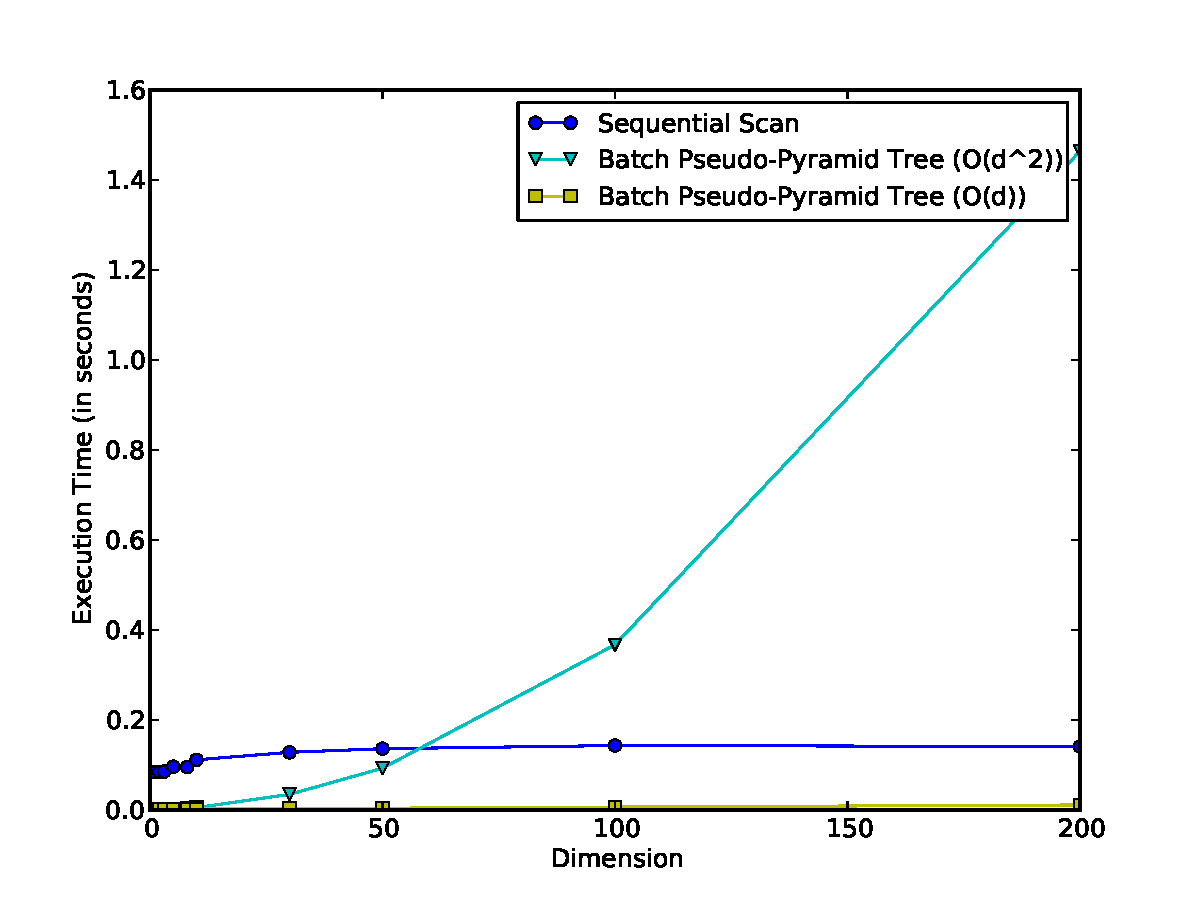
\includegraphics[scale=0.5]{figures/performance_analysis/iteration_2/new_pseudo-pyramid_hash_performance.pdf}
	\caption{\texttt{insert} Performance on Random Uniformly Distributed Datasets of Varying Dimensions}
	\label{fig:new-pseudo-pyramid-hash}
\end{figure}

\subsection{SSE Optimisation}

Since optimising the hashing function resulted in a massive speed increase, it was decided that the function would be parallelised using SSE. Considering point equality is used throughout all the index structures and will be executed many times if there are large buckets in the Pseudo-Pyramid Tree, it is worth optimising to see if there is any major speed-up. Point equality, like the hashing function, is an $O(d)$ operation. In both operations, there is loop which iterates once for each dimension, where each iteration is independent of the others. If 32-bit floating point numbers are used, then four dimensions can be processed at once using 128 bit SSE registers. Since each operation does not spend their entire time hashing or comparing points, it is not expected that a speedup of four can be achieved.

Table \ref{tab:pseudo-pyramid-sse} shows the execution times of the Pseudo-Pyramid Tree with and without SSE optimisation for the hash function and point equality. Across all three operations, the speedup averages to approximately $1.97$ when there are 200 dimensions. Note that if the number of dimensions is less than four, there is little benefit using the 128-bit SSE registers, so the structure uses the sequential hashing function and point equality check.

\begin{table}
	\centering
	\begin{tabular}{|l|l|l|}
		\hline
		\textbf{Operation} & \textbf{Without SSE} & \textbf{With SSE} \\
		\hline
		Insert & 0.0112199 & 0.00674333 \\
		Delete & 0.00625336 & 0.00313489 \\
		Point Query & 0.0076015 & 0.00298432 \\
		\hline
	\end{tabular}
	\caption{Total Execution Time (in seconds) of Batch Pseudo-Pyramid Tree With and Without SSE Optimisation (200D Randomly Uniform Dataset, 10,000 operations each)}
	\label{tab:pseudo-pyramid-sse}
\end{table}

\subsection{Bucket Pseudo-Pyramid Tree}

The index-based variants require the CPU has to fetch two elements from main memory for each point in a bucket -- the index of a point and the point itself. This also results in more random accesses in the single point array, potentially causing more cache misses, because a bucket's indices may point to distant parts of the large point array. Furthermore, having a large point array makes \texttt{delete} operations difficult to perform cheaply.

The Bucket Pseudo-Pyramid Tree implementation does not use a single array to store the points. Instead of buckets containing an array of point indices, it has an array of actual points. The goal of this variant is to increase \textbf{cache coherency} when searching a bucket, since the point array can be searched sequentially and only one memory read is required. No cleanup procedure is necessary because the memory for a point is released immediately after it's removed, by simply erasing it from the corresponding bucket's array (which is much smaller than an array containing \textit{all} the points). However, \texttt{delete} is still an $O(n)$ operation since the worst case is when a single bucket stores all $n$ points.

The order the points are stored in a bucket do not matter, the C++ \textit{erase-remove} idiom has been used to delete elements from the bucket arrays. This idiom swaps the element to delete with the last element in the array, removing the desired element when it's at the end of the array. This means there is no need to move any elements in the array to fill the gap created by removing an element, since the element removed is always at the end of the array.

\subsection{Splay Pseudo-Pyramid Tree}

Unlike the other implementations, the Splay Pseudo-Pyramid Tree does not use a hash map as the underlying one-dimensional index structure, but a splay tree. The splay tree is a self-adjusting variant of the binary search tree that uses a \textit{splaying} operation (a heuristic) to allow faster access to recently accessed elements. \cite{splay-tree}. The splaying operation achieves this by performing a series of tree rotations that move a given node up to the root of the tree. Through amortised analysis and empirical experiments, it has been shown splay trees can be more efficient than standard binary trees for a series of non-random operations \cite{splay-tree}, despite the asymptotic worst case bound being worse than binary search trees.

Nodes in the Splay Pseudo-Pyramid Tree correspond to individual buckets in the Bucket Pseudo-Pyramid Tree, meaning each node can store multiple points. Since the splay tree is implemented as a collection of heap-allocated nodes with pointers to link them, deletions are cheap as a low amount of memory needs to be de-allocated per \texttt{delete} operation. The aim is that this, combined with the self-adjusting nature of the splay tree, will produce a Pseudo-Pyramid Tree implementation that is more efficient for non-random operations used in real applications.

\subsection{Performance Timings}

All variants of the Pseudo-Pyramid Tree hash $d$-dimensional points to a one-dimensional value, which is used as a key to search for a given point in a one-dimensional structure. What varies is how points are deleted and which underlying one-dimensional structure is used. The Batch Pseudo-Pyramid Tree never releases memory after points are removed. For dynamic data which changes frequently, this may cause the machine to run out of memory, so this variant will not be explored any further.

The remaining variants of the Pseudo-Pyramid and the two baselines, Sequential Scan and Octree, were timed with the full collection of synthetic and real datasets. $B = 300000$ and $R=3000$ was used as parameters for the Pseudo-Pyramid Trees. This means the Defragmented and Rebuild Pseudo-Pyramid Tree defragment and rebuild respectively when 3001 elements have been marked for deletion.

Table \ref{tab:perf1-dimensionality} contains the \textit{total} runtime of \texttt{insert}, \texttt{delete} and point query for uniformly randomly generated points for the analysed structures. When ``-" is shown instead of the number of seconds, it means that the performance test could not finish due to the machine running out of memory. Plots with dimension against execution time are shown for \texttt{insert} and \texttt{remove} in Figure \ref{fig:perf1-dimensionality}. The execution times for skewed and clustered data was almost identical to the uniformly random datasets; for the sake of brevity, the tables and plots for these datasets have been placed in Appendix \ref{chap:supp-material}.

\begin{table}
	\centering
	\makebox[\textwidth][c]{%
		\begin{tabular}{|r|r|l|l|l|l|l|l|l|l|}
			\hline
			\multicolumn{2}{|c}{} & \multicolumn{8}{|c|}{\textbf{Dimensionality}} \\
			\hline
			\textbf{Structure} & \textbf{Operation} & 1 & 2 & 3 & 5 & 10 & 50 & 100 & 200 \\
			\hline
			\multirow{3}{*}{Sequential Scan} & Insert & TODO & TODO & TODO & TODO & TODO & TODO & TODO & TODO \\
				& Delete & TODO & TODO & TODO & TODO & TODO & TODO & TODO & TODO \\
				& PQuery & TODO & TODO & TODO & TODO & TODO & TODO & TODO & TODO \\
			\hline			
			\multirow{3}{*}{Octree} & Insert & TODO & TODO & TODO & TODO & TODO & TODO & TODO & TODO \\
				& Delete & TODO & TODO & TODO & TODO & TODO & TODO & TODO & TODO \\
				& PQuery & TODO & TODO & TODO & TODO & TODO & TODO & TODO & TODO \\
			\hline			
			\multirow{3}{*}{Defragmented PPT} & Insert & TODO & TODO & TODO & TODO & TODO & TODO & TODO & TODO \\
				& Delete & TODO & TODO & TODO & TODO & TODO & TODO & TODO & TODO \\
				& PQuery & TODO & TODO & TODO & TODO & TODO & TODO & TODO & TODO \\
			\hline
			\multirow{3}{*}{Rebuild PPT} & Insert & TODO & TODO & TODO & TODO & TODO & TODO & TODO & TODO \\
				& Delete & TODO & TODO & TODO & TODO & TODO & TODO & TODO & TODO \\
				& PQuery & TODO & TODO & TODO & TODO & TODO & TODO & TODO & TODO \\
			\hline
			\multirow{3}{*}{Bucket PPT} & Insert & TODO & TODO & TODO & TODO & TODO & TODO & TODO & TODO \\
				& Delete & TODO & TODO & TODO & TODO & TODO & TODO & TODO & TODO \\
				& PQuery & TODO & TODO & TODO & TODO & TODO & TODO & TODO & TODO \\
			\hline
			\multirow{3}{*}{Splay PPT} & Insert & TODO & TODO & TODO & TODO & TODO & TODO & TODO & TODO \\
				& Delete & TODO & TODO & TODO & TODO & TODO & TODO & TODO & TODO \\
				& PQuery & TODO & TODO & TODO & TODO & TODO & TODO & TODO & TODO \\
			\hline
		\end{tabular}
	}%

	\caption{Total Execution Time (in seconds) of Each Operation for Varying Number of Dimensions in Uniformly Distributed Synthetic Dataset}
	\label{tab:perf1-dimensionality}
\end{table}

\begin{figure}
	\begin{center}
		\begin{subfloat}[\texttt{insert}\label{fig:perf1-dimensionality-insert}]{%
			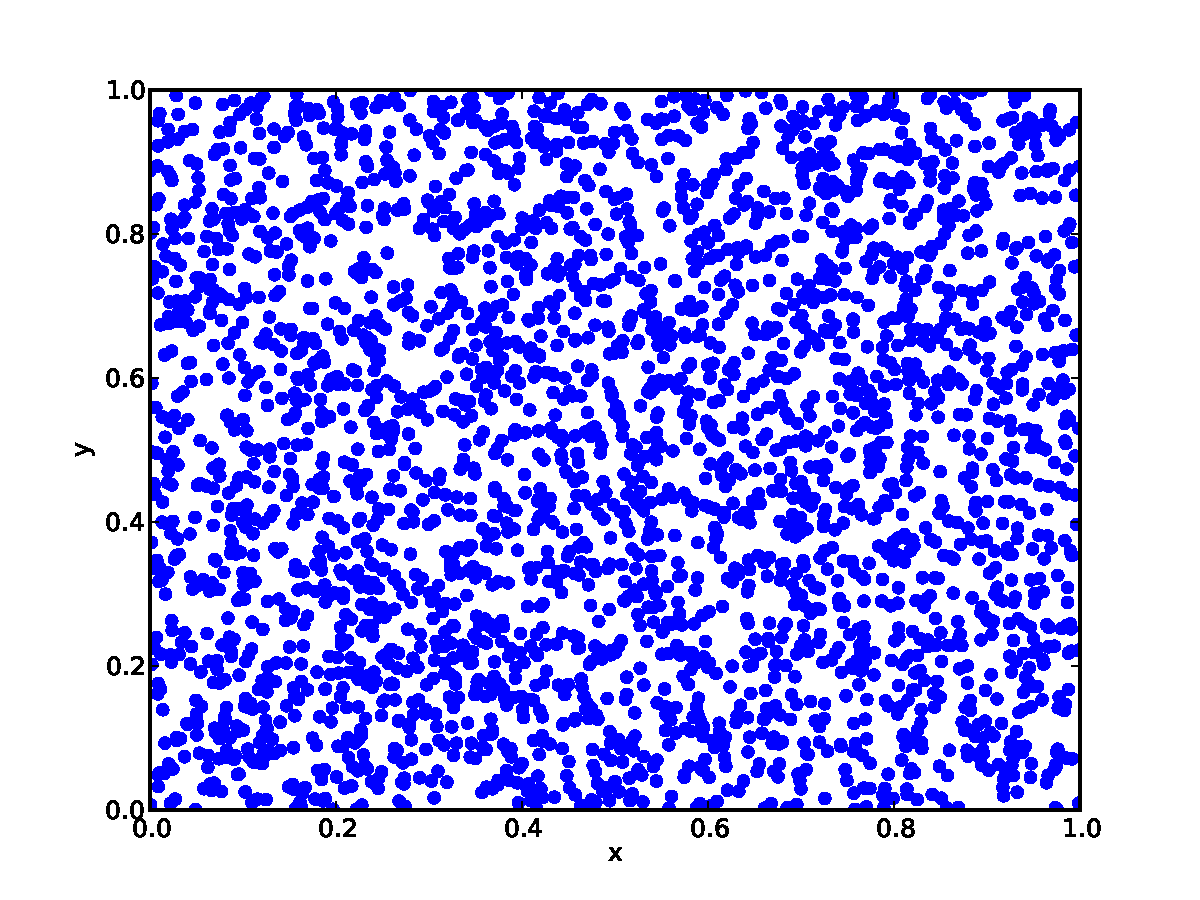
\includegraphics[scale=0.25]{figures/uniform_distribution.pdf}
		}
		\end{subfloat}~
		\begin{subfloat}[\texttt{remove}\label{fig:perf1-dimensionality-remove}]{%
			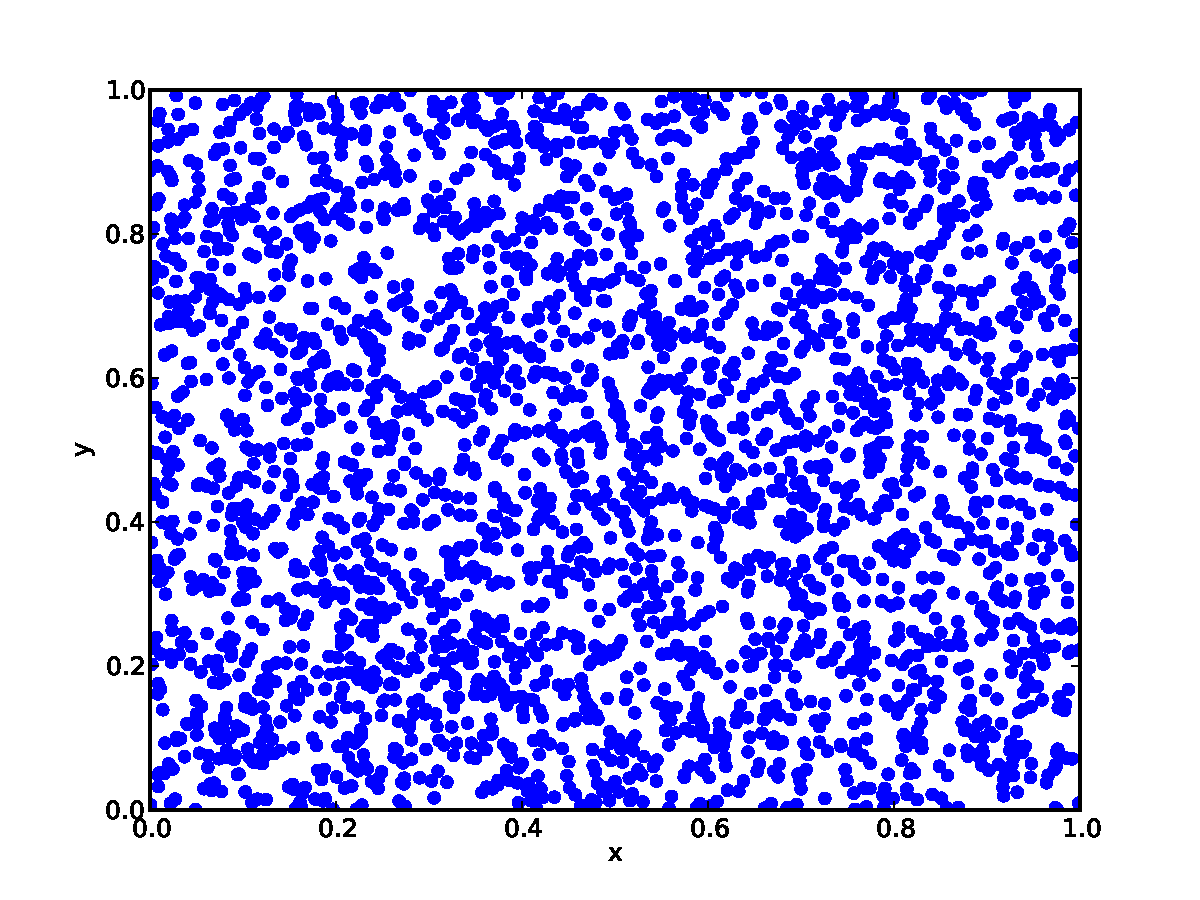
\includegraphics[scale=0.25]{figures/uniform_distribution.pdf}
		}
		\end{subfloat}~
	\end{center}

	\caption{Index Structure Performance With Respect To Dimensionality (10,000 Points from Uniform Distribution Synthetic Dataset)}
	\label{fig:perf1-dimensionality}
\end{figure}

The three plots show that dimensionality has little effect on \textit{insert} and point queries for Sequential Scan. \texttt{delete}'s execution time increases as $d$ does, most likely because higher $d$ means more data has to be moved when a point is deleted from the underlying array. As expected, the Octree takes exponentially longer as $d$ increases, due to the exponential increase in nodes at each level ($2^d$ children per node). After 10 the number of excessive nodes was so high that the performance tests crashed due to there being no more memory to allocate.

All Pseudo-Pyramid Tree variants have similar speeds for \texttt{insert} and point queries, which significant outperforms Sequential Scan and Octree. However, the performance of the trees decreases as $d$ increases. The $O(n^2)$ defragmentation procedure used by the Defragmented Pseudo-Pyramid Tree causes it to be the slowest structure for deleting points, taking almost twice as long as Sequential Scan. Rebuild Pseudo-Pyramid tree is better, but still much slower than the Bucket or Splay Pseudo-Pyramid Tree variants, which have the fastest deletion speed. This is because TODO.

\begin{table}
	\centering
	\makebox[\textwidth][c]{%
		\begin{tabular}{|r|r|l|l|l|l|}
			\hline
			\multicolumn{2}{|c}{} & \multicolumn{4}{|c|}{\textbf{Points in Dataset}} \\
			\hline
			\textbf{Structure} & \textbf{Operation} & 10,000 & 100,000 & 500,000 & 1,000,000 \\
			\hline
			\multirow{3}{*}{Sequential Scan} & Insert & TODO & TODO & TODO & TODO \\
				& Delete & TODO & TODO & TODO & TODO \\
				& PQuery & TODO & TODO & TODO & TODO \\
			\hline
			\multirow{3}{*}{Octree} & Insert & TODO & TODO & TODO & TODO \\
				& Delete & TODO & TODO & TODO & TODO \\
				& PQuery & TODO & TODO & TODO & TODO \\
			\hline
			\multirow{3}{*}{Defragmented PPT} & Insert & TODO & TODO & TODO & TODO \\
				& Delete & TODO & TODO & TODO & TODO \\
				& PQuery & TODO & TODO & TODO & TODO \\
			\hline
			\multirow{3}{*}{Rebuild PPT} & Insert & TODO & TODO & TODO & TODO \\
				& Delete & TODO & TODO & TODO & TODO \\
				& PQuery & TODO & TODO & TODO & TODO \\
			\hline
			\multirow{3}{*}{Bucket PPT} & Insert & TODO & TODO & TODO & TODO \\
				& Delete & TODO & TODO & TODO & TODO \\
				& PQuery & TODO & TODO & TODO & TODO \\
			\hline
			\multirow{3}{*}{Splay PPT} & Insert & TODO & TODO & TODO & TODO \\
				& Delete & TODO & TODO & TODO & TODO \\
				& PQuery & TODO & TODO & TODO & TODO \\
			\hline
		\end{tabular}
	}%

	\caption{Total Execution Time (in seconds) of Each Operation for Varying Number of Points in Uniformly Distributed Synthetic Dataset}
	\label{tab:perf1-size}
\end{table}

\begin{figure}
	\begin{center}
		\begin{subfloat}[\texttt{insert}\label{fig:perf1-size-insert}]{%
			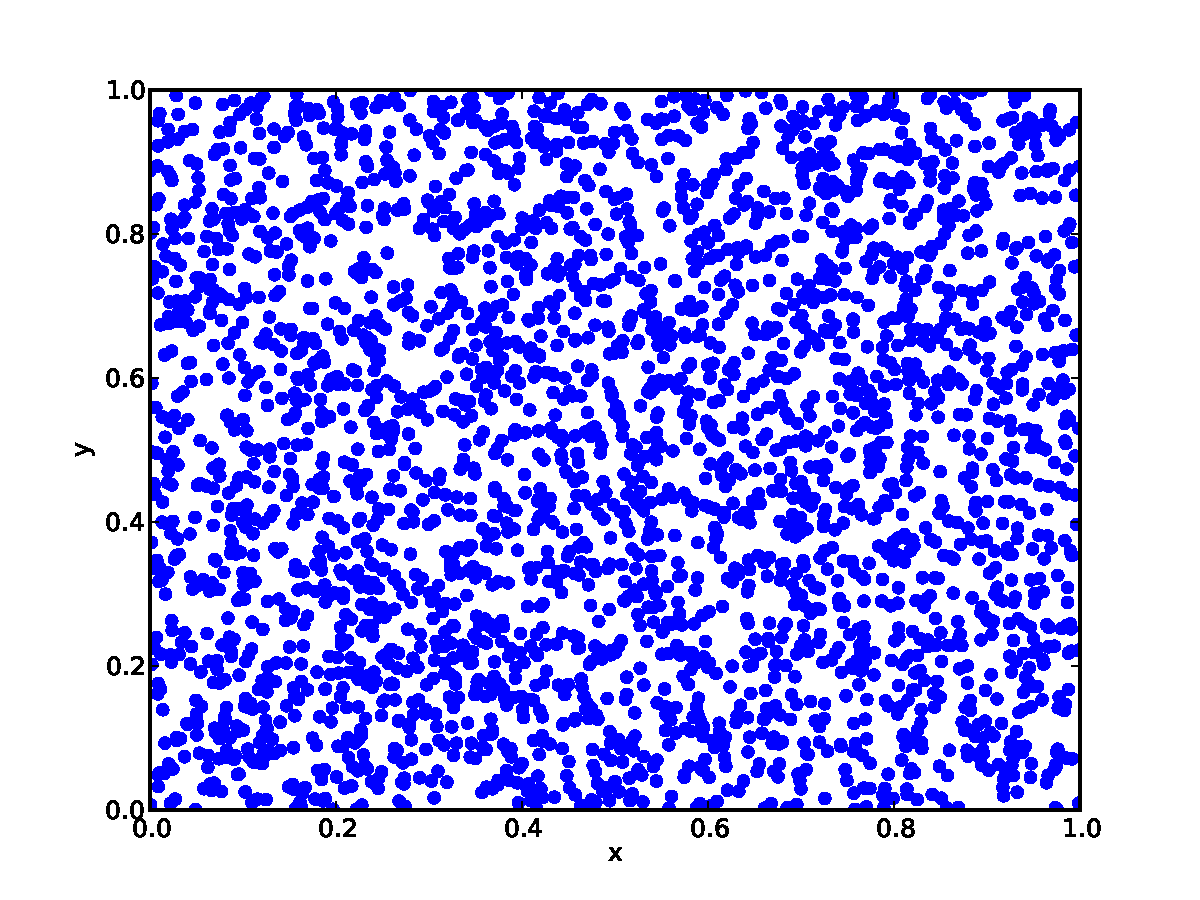
\includegraphics[scale=0.25]{figures/uniform_distribution.pdf}
		}
		\end{subfloat}~
		\begin{subfloat}[\texttt{remove}\label{fig:perf1-size-remove}]{%
			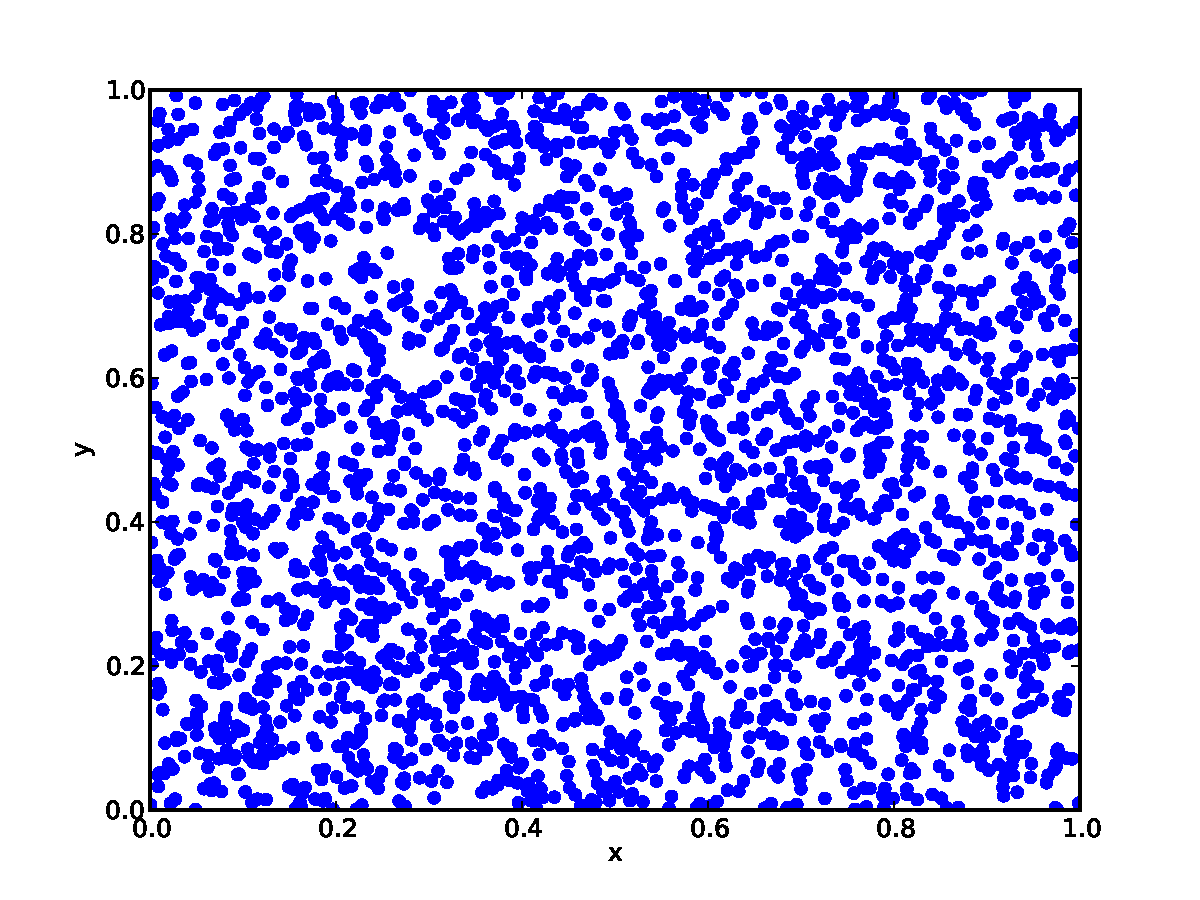
\includegraphics[scale=0.25]{figures/uniform_distribution.pdf}
		}
		\end{subfloat}~
	\end{center}

	\caption{Index Structure Performance With Respect To Dataset Size (10,000 Points from Uniform Distribution Synthetic Dataset)}
	\label{fig:perf1-size}
\end{figure}

Execution times for the 16 dimension dataset of varying size are displayed in Table \ref{tab:perf1-size} and Figure \ref{fig:perf1-size}. From the plots, it appears the average time it takes to perform a point query and the other operations for Sequential Scan roughly grows linearly with $n$. This is to be expected, due to the complexity of its operations being $O(n)$. The average time for both operations with the Pseudo-Pyramid Tree variants grow very slowly as $n$ increases. This is likely because an operation's average complexity is $O(d)$ and dataset size only affects the performance of these operations if the tree's buckets become crowded with many points (as the buckets have to be searched to find the point).

\texttt{delete} in the Defragmented and Rebuild Pseudo-Pyramid Trees grow rapidly as $n$ is increased. Despite the defragmentation procedure being $O(n^2)$, the operation's execution appears to have linear growth (albeit with a higher constant factor than Sequential Scan). Perhaps this worst case bound was simply not reached in the tests, or there is some compiler optimisation at work which reduces this complexity.

Storing separate point arrays for each bucket, instead of using one large array to store all the points, can increase performance. This is shown by the bucket and splay variants providing faster \texttt{insert} and point query operations than the index-based variants. As expected, this is due to an increased cache hit rate. Table \ref{tab:perf1-cache-hit-rate} displays the cache miss rate (rounded to 2 decimal places) for each Pseudo-Pyramid Tree implementation. Notice how the two implementations which store indices in buckets have a greater cache miss rate. 

\begin{table}
	\centering
	\begin{tabular}{|l|l|}
		\hline
		\textbf{Structure} & \textbf{Cache Miss Rate (\%)} \\
		\hline
		Defragmented Pseudo-Pyramid Tree & 7.52 \\
		Rebuild Pseudo-Pyramid Tree & 4.65 \\
		Bucket Pseudo-Pyramid Tree & 0.13 \\
		Splay Pseudo-Pyramid Tree & 0.29 \\
		\hline
	\end{tabular}
	\caption{Cache Hit Rate for \texttt{insert} Operations with Pseudo-Pyramid Variants (200D Randomly Uniform Dataset, 10,000 operations each)}
	\label{tab:perf1-cache-hit-rate}
\end{table}

The differences in speed between the bucket and splay variants is small, but the Bucket Pseudo-Pyramid Tree outperforms the Splay Tree with most datasets. Again, this may be due to having a lower cache miss rate. With severely skewed synthetic data, the splay variant is \textit{slightly} faster, but the speed increase is negligible. This could be an indication that self-adjusting structures are useful for heavily skewed data however, highlighting an area for further study. TODO: refer to table

\begin{table}
	\centering
	\makebox[\textwidth][c]{%
		\begin{tabular}{|r|r|l|l|l|}
			\hline
			\multicolumn{2}{|c}{} & \multicolumn{3}{|c|}{\textbf{Dataset}} \\
			\hline
			\textbf{Structure} & \textbf{Operation} & \textbf{Astrophysics} & \textbf{Hurricane Isabel} & \textbf{Armadillo Mesh} \\
			\hline
			\multirow{4}{*}{Sequential Scan} & Insert & TODO & TODO & TODO \\
				& Delete & TODO & TODO & TODO \\
				& PQuery & TODO & TODO & TODO \\
				& Random Operation List & TODO & TODO & TODO \\
			\hline
			\multirow{4}{*}{Octree} & Insert & TODO & TODO & TODO \\
				& Delete & TODO & TODO & TODO \\
				& PQuery & TODO & TODO & TODO \\
				& Random Operation List & TODO & TODO & TODO \\
			\hline
			\multirow{4}{*}{Defragmented PPT} & Insert & TODO & TODO & TODO \\
				& Delete & TODO & TODO & TODO \\
				& PQuery & TODO & TODO & TODO \\
				& Random Operation List & TODO & TODO & TODO \\
			\hline
			\multirow{4}{*}{Rebuild PPT} & Insert & TODO & TODO & TODO \\
				& Delete & TODO & TODO & TODO \\
				& PQuery & TODO & TODO & TODO \\
				& Random Operation List & TODO & TODO & TODO \\
			\hline
			\multirow{4}{*}{Bucket PPT} & Insert & TODO & TODO & TODO \\
				& Delete & TODO & TODO & TODO \\
				& PQuery & TODO & TODO & TODO \\
				& Random Operation List & TODO & TODO & TODO \\
			\hline
			\multirow{4}{*}{Splay PPT} & Insert & TODO & TODO & TODO \\
				& Delete & TODO & TODO & TODO \\
				& PQuery & TODO & TODO & TODO \\
				& Random Operation List & TODO & TODO & TODO \\
			\hline
		\end{tabular}
	}%

	\caption{Total Execution Time (in seconds) of Each Operation for 500,000 Points Sampled From Real Datasets}
	\label{tab:perf1-real}
\end{table}

Table \ref{tab:perf1-real} shows the runtime of each operation on the real evaluation datasets, measured using the Insert-Query-Delete operation list.TODO: remarks on it

\subsection{Profiling Results}

CPU and heap profiling was performed on each structure to determine where the performance bottlenecks are and how much memory each structure uses. Table \ref{fig:perf1-profiling} shows which functions took the majority of the execution time for each structure, as well as how much heap memory the structure consumed when storing all of the input dataset's points. The dataset used contained 10,000 10D uniformly random points and the CPU profiling was performed over the Insert-Query-Delete operation list.

\begin{table}
	\centering
	\makebox[\textwidth][c]{%
		\begin{tabular}{|l|l|l|}
			\hline
			\textbf{Structure} & \textbf{Peak Heap Memory (MB)} & \textbf{Dominant Function (\% Total Time Spent)} \\
			\hline
			Sequential Scan & 4.1 & \texttt{pointExists()} (34.4\%) \\
			Defragmented PPT & 10.9 & \texttt{defragment()} (76.6\%)\\
			Rebuild PPT & 16.8 & \texttt{rebuild()} (60.7\%)\\
			Bucket PPT & 11.2 & \texttt{remove()} (19.2\%) \\
			Splay PPT & 11.8 & \texttt{insert()} (47.2\%) \\
			\hline
		\end{tabular}
	}%
	\caption{CPU and Heap Profiling Statistics for Insert-Query Delete Operation List with 500,000 Points from 16D Synthetic Dataset}
	\label{tab:perf1-profiling}
\end{table}

TODO: analysis

\subsection{Impact of Bucket Size}

Work gone into increasing the speed of the Pseudo-Pyramid Tree by exploring different variants of the structure's implementation. This has worked to greatly accelerate the structure for most of the evaluation datasets. However, when testing on the astrophysics dataset, the speedup when compared to Sequential Scan seemed to be quite low. For example, $500,000$ insertion operations with the astrophysics dataset takes TODO seconds with Sequential Scan and TODO seconds with the Bucket Pseudo-Pyramid Tree, meaning a speedup of $\frac{TODO}{TODO} \approx TODO$ has been achieved. Considering there exist algorithms which can perform search in $O(log_2 n)$ time, this raised the question of why the speedup is so low for the astrophysics dataset.

Despite hashing a point taking $O(d)$ time, point queries will take much longer if there are large numbers of points in buckets. If each bucket contains exactly one point, then the complexity approaches $O(d)$. On the other extreme, where a single bucket contains all points, the complexity becomes $O(n)$. The number of points in a bucket, or \textit{bucket size}, is one of the most important factors to consider when analysing the performance of hash-based index structures. A ``good" hashing function tries to achieve an amortised running time of $O(1)$ by ensuring only one or two points are mapped to the same hash value.

The mean, standard deviation, minimum and maximum bucket size has been used to determine if bucket size is the reason the Pseudo-Pyramid Tree is so slow for the astrophysics dataset. Table \ref{tab:perf1-bucket-stats} shows these statistics when the Pseudo-Pyramid Tree is storing points from one synthetic dataset and all the real datasets.

\begin{table}
	\centering
	\begin{tabular}{|l|l|l|l|l|l|}
		\hline
		& & \multicolumn{4}{c|}{\textbf{Bucket Size Statistics}} \\
		\hline
		\textbf{Dataset} & \textbf{Time to Insert (sec)} & \textbf{Average} & \textbf{St. Dev} & \textbf{Min} & \textbf{Max} \\
		\hline
		500,000 16D Random Points & TODO & 1.0312 & 0.115177 & 1 & 4 \\
		500,000 Astrophysics Points & TODO & 3586.57 & 24,528 & 1 & 235,260 \\
		500,000 Hurricane Isabel Points & TODO & 17,323.66 & 83,533 & 1 & 293,949 \\
		435,544 3D Armadillo Mesh Points & TODO & 19.1465 & 14.9386 & 1 & 187 \\
		\hline
	\end{tabular}
	\caption{Statistics on Bucket Size with Pseudo-Pyramid Tree Based on Dataset}
	\label{tab:perf1-bucket-stats}
\end{table}

TODO: remarks on stats in above table

TODO: why is bucket size so high????????????

\subsection{Summary}

All Pseudo-Pyramid tree invariants greatly outperform the two baselines, with the Octree failing to store large numbers of points or points with more than 10 dimensions due to exponential memory requirements. The defragmented and rebuild variants of the Pseudo-Pyramid are clearly inferior to batch and splay, being slower for all three operations. While the Splay Pseudo-Pyramid Tree performs the fastest for some datasets, the Bucket Pseudo-Pyramid Tree performs the fastest on the majority of the datasets. Therefore, the Bucket Pseudo-Pyramid Tree will be used for any future evaluations.

With both scientific datasets, all Pseudo-Pyramid Tree variants performed incredibly slowly, due to the nature of the hash function. The next iteration performed more research into decreasing bucket size by using different hashing functions, to determine whether or not hash-based index structures can provide fast point queries for scientific datasets with TODO(nature of data).